%%%%%%%%%%%%%%%%%%%%%%%%%%%%%%%%%%%%%%%%%%%%%%%%%%%
% detectormodeling.tex
%%%%%%%%%%%%%%%%%%%%%%%%%%%%%%%%%%%%%%%%%%%%%%%%%%%
\label{sec:detmod}

\subsection{\textbf{Detector Modeling}}

\subsubsection{Introduction}
A key component of \Gfour{} is the geometry modeler~\cite{detmodeling:modeler},
which provides a wide variety of tools and solutions for describing geometry 
setups from simple to highly complex.  Geometrical models of the LHC detectors,
for instance, easily reach millions of geometrical elements of different kinds
combined together in hierarchical structures.  The geometry modeler provides
techniques by which memory consumption can be greatly reduced, allowing regular 
or irregular patterns to be easily replicated, assembled or reflected.  This, 
combined with navigation and optimization algorithms, allow the efficient 
computation of intersections of simulated tracks with the elements composing
any geometry setup.

Recent extensions of the geometry modeler include specialized navigation
techniques and optimization algorithms to aid medical simulation studies. 
This has allowed complex geometrical models of the human body to be developed.
Extensions also include parallel navigation and tracking in layered geometries
which allow geometry setups to be superimposed on one another with minimal 
impact on CPU time.

\subsubsection{Navigation in geometries} \label{sec:nav}
The recent addition featuring ``parallel geometries'' allows the definition and
treatment of more than one independent geometry in parallel for different 
potential uses, and exploits the existing enhanced interface provided by the 
navigation system in the \Gfour{} toolkit \cite{detmodeling:parGeom}.  In 
\Gfour{} a geometry setup is in general associated with a navigator which is a
concrete instance of the \gclass{G4Navigator} class.  \gclass{G4Navigator} was 
designed such that several instances of it can be created and coexist; each 
instance can be assigned to a different geometry hierarchy.  The primary 
navigation instance is attached to the ``mass world'' which is the main geometry 
hierarchy in which the material of the setup is described;  this setup is unique
and is used for all physical interactions.

``Parallel world'' geometries may be assigned to the additional navigator objects
and may be used for example as simple ``locators'', independent of the mass 
world, to identify exact positioning in the other geometries of a particular 
point in the global coordinate system.  Each geometry must have an
independent root volume (the world volume), which contains a hierarchy of 
physical volumes.  Volumes in one world may overlap volumes in a different 
world. 

Volumes in a parallel world geometry can be associated with the read-out 
structure of a detector.  In shower parameterization studies, for example, the
simplified read-out geometry of a calorimeter could overlay its more complex
mass geometry.  Parallel worlds are also useful in importance biasing and
scoring of doses and other radiation measures.

Volumes in a parallel world may have material; these are referred to as the
``layered mass geometry''.  In this case, the material defined in a volume in
the parallel world overrides the material defined in the mass world and is 
used for the calculation of physical interactions.  If more than one parallel 
world is overlaid on the mass world, the parallel worlds are examined, in 
reverse order of their creation, to see if any volumes with materials are 
defined in them.  Any such volumes found will override the materials in all 
previously created worlds.  Because volumes in the mass geometry always have 
materials, the material to be used for physical interactions is always 
uniquely defined.

Layered mass geometry offers an alternative way of describing complicated 
shapes that would otherwise require massive boolean operations to combine 
primitive volumes.  Examples include a photo-multiplier system partially 
dipped in a noble liquid and brachytherapy seeds implanted in the CT-scanned 
voxels of a patient.  A voxel refers to a volume element which represents a 
value on a three-dimensional grid.

In addition, different parallel worlds may be assigned to different particle 
types.  Thus, in the case of a sampling calorimeter, the mass world could 
be defined as having only a crude geometry with averaged material, while a 
parallel world would contain the detailed geometry.  The real materials in the
detailed parallel world geometry would be associated only with particle types 
that require accurate tracking, such as muons, while other particle types such
as electrons, positrons and gammas would see crude, less complicated geometry 
for faster simulation.

\subsubsection{Navigation in regular geometries}
When the voxels in a geometry are numerous and of the same size and shape, a 
specialized navigator can take advantage of the regularity to deliver faster
CPU performance.  This is useful in medical physics applications in which there
could be millions of identical volumes comprising a 3-D image of a patient.
% or test phantom.  
In this case the navigator can use a regular grid to easily 
locate the incident particle in the geometry.

In the \Gfour{} implementation 
\gclass{G4Phantom\allowbreak{}Para\allowbreak{}meter\allowbreak{}isation} 
defines the regular structure of the geometry, using the parameters of dimension, 
offset and number of voxels in each of three dimensions.  \gclass{G4RegularNavigation} 
uses this parameterization to directly locate the voxel visited by tracks in the
simulation.  An option is provided which allows boundaries between contiguous
voxels to be skipped if they are of the same material, thus significantly reducing
the number of tracking steps.

Using this method of navigation, CPU speed improvement factors of three to six
have been observed.  This factor holds for pure navigation examples (no physics 
interactions) and for beams of gammas.  For the case of electrons or protons
most of the time is spent on physics instead of navigation and the speed 
improvement is substantially reduced.  Significant savings in memory consumption
(factor of seven) and initialization time (factor of two) were also seen 
\cite{detmodeling:regnav}.

\subsubsection{Exact safety}
The ``isotropic safety'' is the distance to the next volume boundary in any 
direction.  It is calculated by the navigator and is used by the multiple 
scattering process in two distinct ways.  The primary use of the safety is to
limit the lateral displacement in order to avoid crossing a boundary within a
step.  Improved safety values reduce the need for artificial restrictions in 
electron displacement, and enable it to be better simulated at particular values
of the model parameters and production thresholds.  The isotropic safety also 
sometimes influences the step size restriction from multiple scattering.  In the
default configuration of this process it has an effect only if the safety is 
larger than the primary restriction (a fraction of the range), in which case the
safety is used as the step limit.     

The estimation of the isotropic safety was improved for volumes which have 
several child volumes.  Previously only the contents of the current voxel in 
the optimization voxels structure automatically generated at initialization, 
and the boundaries of that voxel were considered.  This resulted in a distance
which could be significantly underestimated.  The new method considers enough 
voxels to obtain a precise value of the safety, while ensuring that the number 
of voxels is limited by the running estimate of the safety value.

As a result, an improved estimate of the safety is available.  This ensures 
that the value of the isotropic safety does not depend strongly on the details
of the voxelization, on the number of child volumes, or on the presence of 
volumes in a remote region of the current volume.  The extra computation cost 
was found to be negligible in a complex simulation.

\subsubsection{Improved verbosity}
The geometry modeler with its current version of the navigator offers an 
enhanced verbosity system which can be used to help developers and users in 
debugging problems or to provide closer monitoring of the execution flow and 
behavior of the navigation system during tracking.  A set of UI commands was 
defined and made available by default in the user application which allows the 
execution flow to be controlled with five different levels of detail:
\begin{verbatim}
/geometry/navigator/verbose [level-number]
 -- Setting run-time verbosity for the geometry
      navigation
    Command having effect -only- if Geant4 has
      been installed with verbose mode
      (G4VERBOSE flag) set!
    Level 0: Silent (default)
    Level 1: Display volume positioning and 
              step lengths
    Level 2: Display step/safety info on point
              locations
    Level 3: Display minimal state at -every-
              step
    Level 4: Maximum verbosity (very detailed!)
\end{verbatim}
A special UI command 
\begin{verbatim}
/geometry/navigator/check_mode [true/false]
\end{verbatim}
was also defined to modify the execution mode of the navigator and perform extra
checks for correctness, or to apply stricter and less tolerant conditions to 
stress precision.  This can help in studying and debugging difficult cases by 
eventually highlighting potential defects in the geometry under consideration.
% \begin{verbatim}
% /geometry/navigator/check_mode [true/false]
%  -- Setting navigator in -check_mode- state
%     (default is false).
%     Command having effect -only- if Geant4
%     has been installed with verbose mode
%     (G4VERBOSE flag) set!
% \end{verbatim}
An additional UI command
\begin{verbatim}
/geometry/navigator/push_notify [true/false]
\end{verbatim}
allows the enabling or disabling of notifications from the navigator for 
artificial pushes applied by the navigation system along the track direction in
case tracks get stuck in particular geometries.
% \begin{verbatim}
% /geometry/navigator/push_notify [true/false]
%  -- Setting navigator verbosity push 
%     notifications (default is true).
%     Command having effect -only- if Geant4 
%     has been installed with verbose mode
%     (G4VERBOSE flag) set!
% \end{verbatim}

These new tools, in addition to a more rationalized layout of output messages
for the information provided by the system, contribute to make the navigation
system of \Gfour{} more user-friendly and provide powerful means to users
and developers to improve the quality of their simulation programs.

\begin{figure*}
\centering 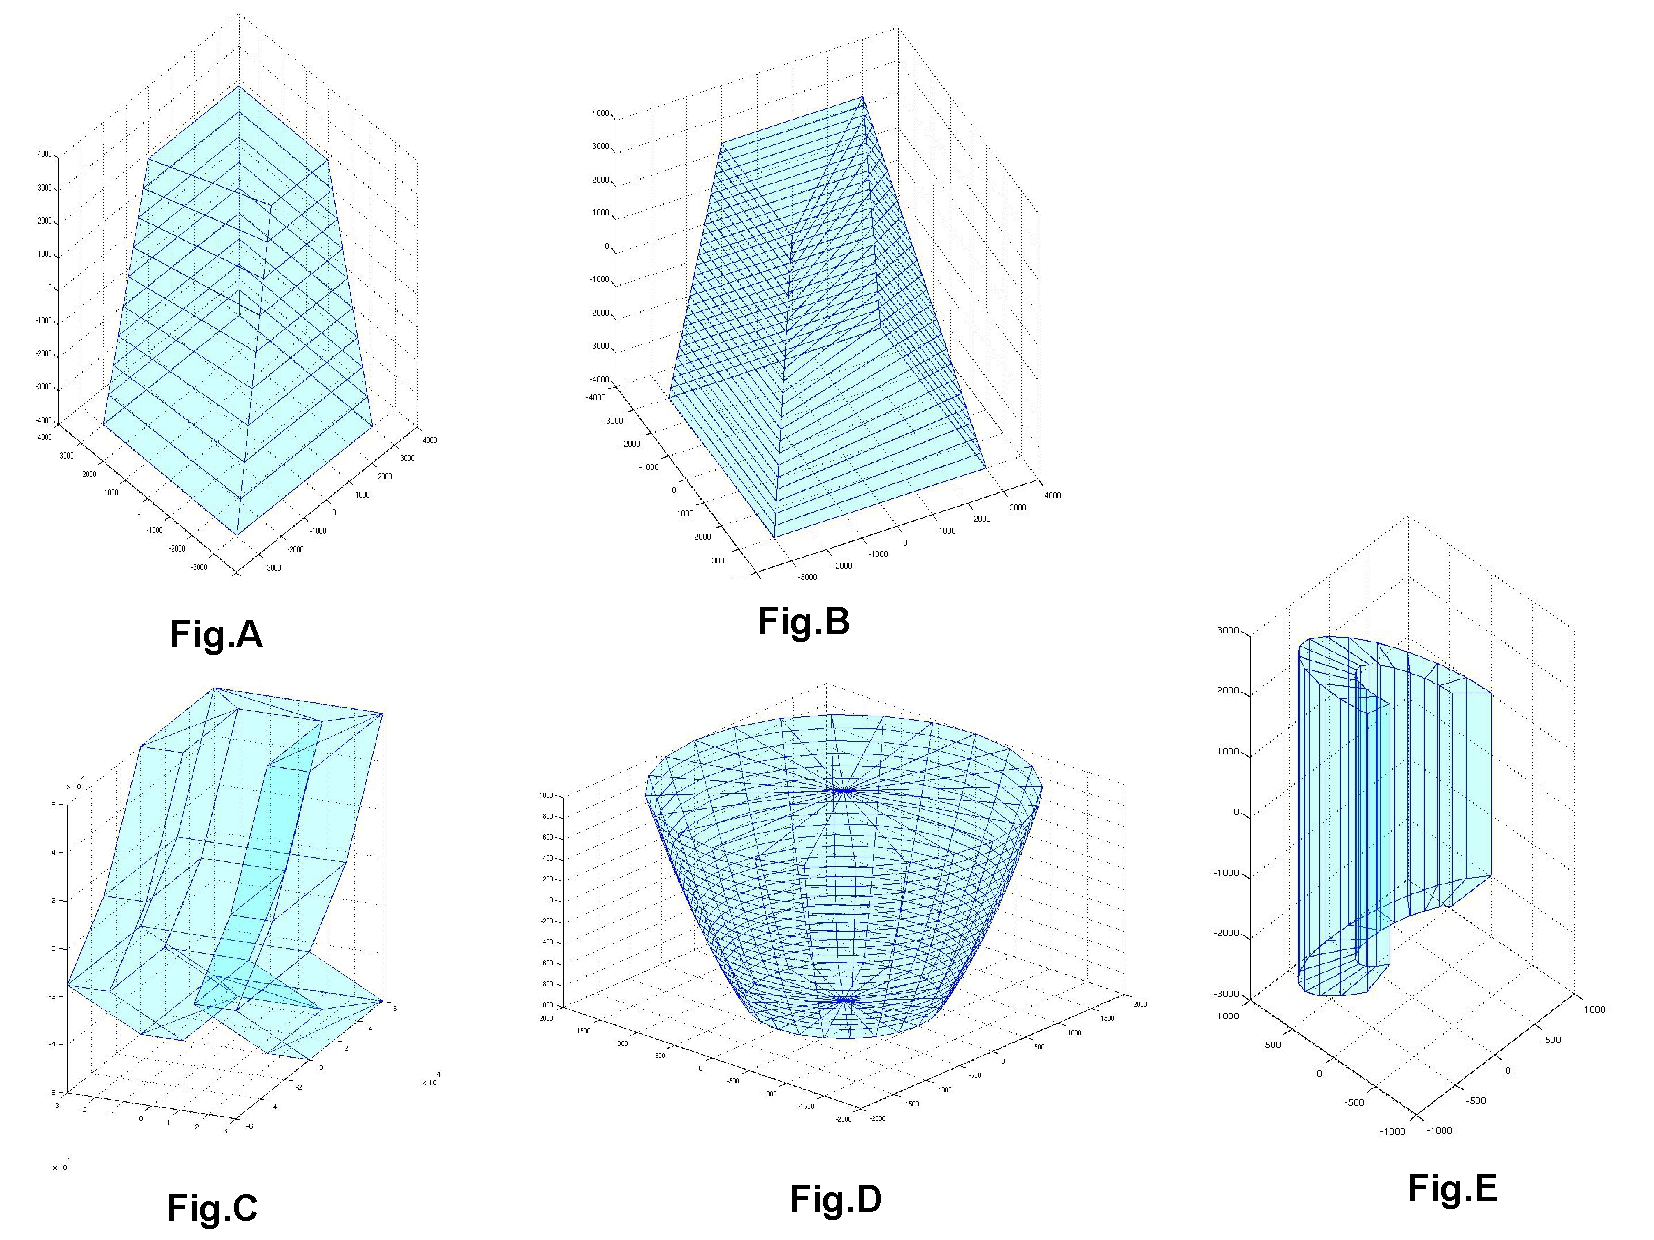
\includegraphics[height=4.0in,width=5.0in]{figures/new_solids.pdf}
\caption{Recent geometrical primitives added in \Gfour{}: generic trapezoid
         (A,B), extruded solid (C), parabolic solid (D), cut tube(E).}
\label{new_solids}
\end{figure*}

\subsubsection{Extensions to geometrical primitives}
Since \Gfour{} release series 8, new geometrical primitives, \gclass{G4GenericTrap}, 
\gclass{G4ExtrudedSolid}, \gclass{G4Paraboloid} and \gclass{G4CutTubs}, have been
part of the toolkit and are shown in Figure~\ref{new_solids}.

\gclass{G4GenericTrap} is an arbitrary trapezoid with up to four vertices lying
in each of two parallel planes at -hz and +hz perpendicular to the $z$ axis.  
Vertices are specified by their $x,y$ coordinates.  Points may be identical in 
order to create shapes with fewer than eight vertices; the only limitation is to
have at least one triangle at +hz or -hz.  The lateral surfaces are not necessarily 
planar and in that case they are represented by a surface that linearly changes
from the edge at -hz to the corresponding edge at +hz.  This represents a 
sweeping surface with a twist angle linearly dependent on $z$, which is different
from the twisted solids which have surfaces described by an equation depending on
a constant twist angle.  In Figure \ref{new_solids}A a \gclass{G4GenericTrap} 
with eight vertices and a twist is shown; Figure \ref{new_solids}B shows a
\gclass{G4GenericTrap} with collapsed vertices and a twist.

\gclass{G4ExtrudedSolid} (Figure \ref{new_solids}C) is a solid obtained by the
extrusion of an arbitrary polygon in the defined $z$ sections.  Each $z$ section
is defined by a $z$-coordinate, an offset in the $x,y$-plane and a factor by
which to scale the polygon at the given $z$ coordinate.  Each section in $z$ of
the \gclass{G4ExtrudedSolid} is a scaled version of the same polygon.  A second,
simplified constructor for the special case of a solid with only two
$z$-sections is also provided.

\gclass{G4Paraboloid} (Figure \ref{new_solids}D) is a solid with a parabolic
profile and possible cuts along the $z$ axis at +hz and -hz, with the cut planes 
perpendicular to the $z$ axis.  To construct the parabolic profile, the 
following equation is used:
\begin{verbatim}
  Z=a* (x*x+y*y)^2+b
\end{verbatim}
with real coefficients $a$ and $b$; the coefficients are calculated from given
radii at +hz and -hz.

\gclass{G4CutTubs} (Figure \ref{new_solids}E) is a tube or cylindrical section
with cuts applied in $z$.  These cuts are planes defined by a normal vector 
pointing outside the tube (cylindrical section) and intersect the $z$ axis at a
given point +hz or (and) -hz.

An important and rather useful construct for shapes delimited by any kind of 
complex surface is offered by the \gclass{G4TessellateSolid} class, which allows
complex geometrical shapes to be described by approximating their surfaces as a
set of planar facets (triangles), with tunable resolution.  This technique can
be used for importing geometries from CAD systems to generate surface-bounded 
solids.  Recent developments during the implementation of the Unified Solids
library~\cite{detmodeling:USolids}, provide considerably improved CPU 
performance, making it possible to use such constructs for very detailed and 
realistic descriptions of surfaces, while optimally scaling with the number of 
facets in use.  A sample \gclass{G4TessellateSolid} is shown in 
Figure \ref{tessellated_cpu}.
 
Unified Solids have been available since \Gfour{} 10.0 as experimental 
alternatives to the traditional geometrical primitives.  The aim is to offer
an independent library of such solids to replace the traditional primitives.

Cloning of all geometrical primitives has been possible since release 9.4, 
with the definition of appropriate copy constructors and assignment operators.
This functionality is required when running in multithreaded mode when 
parameterized geometries are used.  All solids also have the ability to compute
their own surface area and geometrical volume:
\begin{verbatim}
  G4double G4VSolid::GetSurfaceArea()
  G4double G4VSolid::GetCubicVolume() .
\end{verbatim}
A solid's surface area and geometrical volume are estimated using Monte Carlo
sampling methods when it is not possible to compute them with mathematical 
formulae;  in such cases the accuracy can be tuned in case the default does not
provide sufficient precision.  Computed values are expressed in internal units
and are cached for reuse.  In a detector setup, these utilities allow for the
calculation of the overall mass of the setup for a specific logical volume:
\vspace{2.0cm}

\begin{verbatim}
G4double
G4LogicalVolume::GetMass(G4bool forced=false,
                     G4bool propagate=true,
                     G4Material* parMaterial=0) .
\end{verbatim}
The mass of the logical volume tree expressed in internal units is computed
from the estimated geometrical volume of each solid and material associated
with the logical volume and, by default, its daughters.  The returned value
is also cached in this case and can be used for successive calls, unless
recomputation is forced by providing 'true' for the boolean argument (i.e. 
in case the geometry setup has changed after the previous call).  By setting
the ``propagate'' Boolean flag to 'false' only the mass of the current logical 
volume is returned (with the volume occupied by the daughter volumes 
subtracted).  An optional argument ``parMaterial'' can be used to specify a 
custom material for a specific logical volume; the argument is also used 
internally to consider cases of geometrical parameterization by material. 

\begin{figure}
\centering 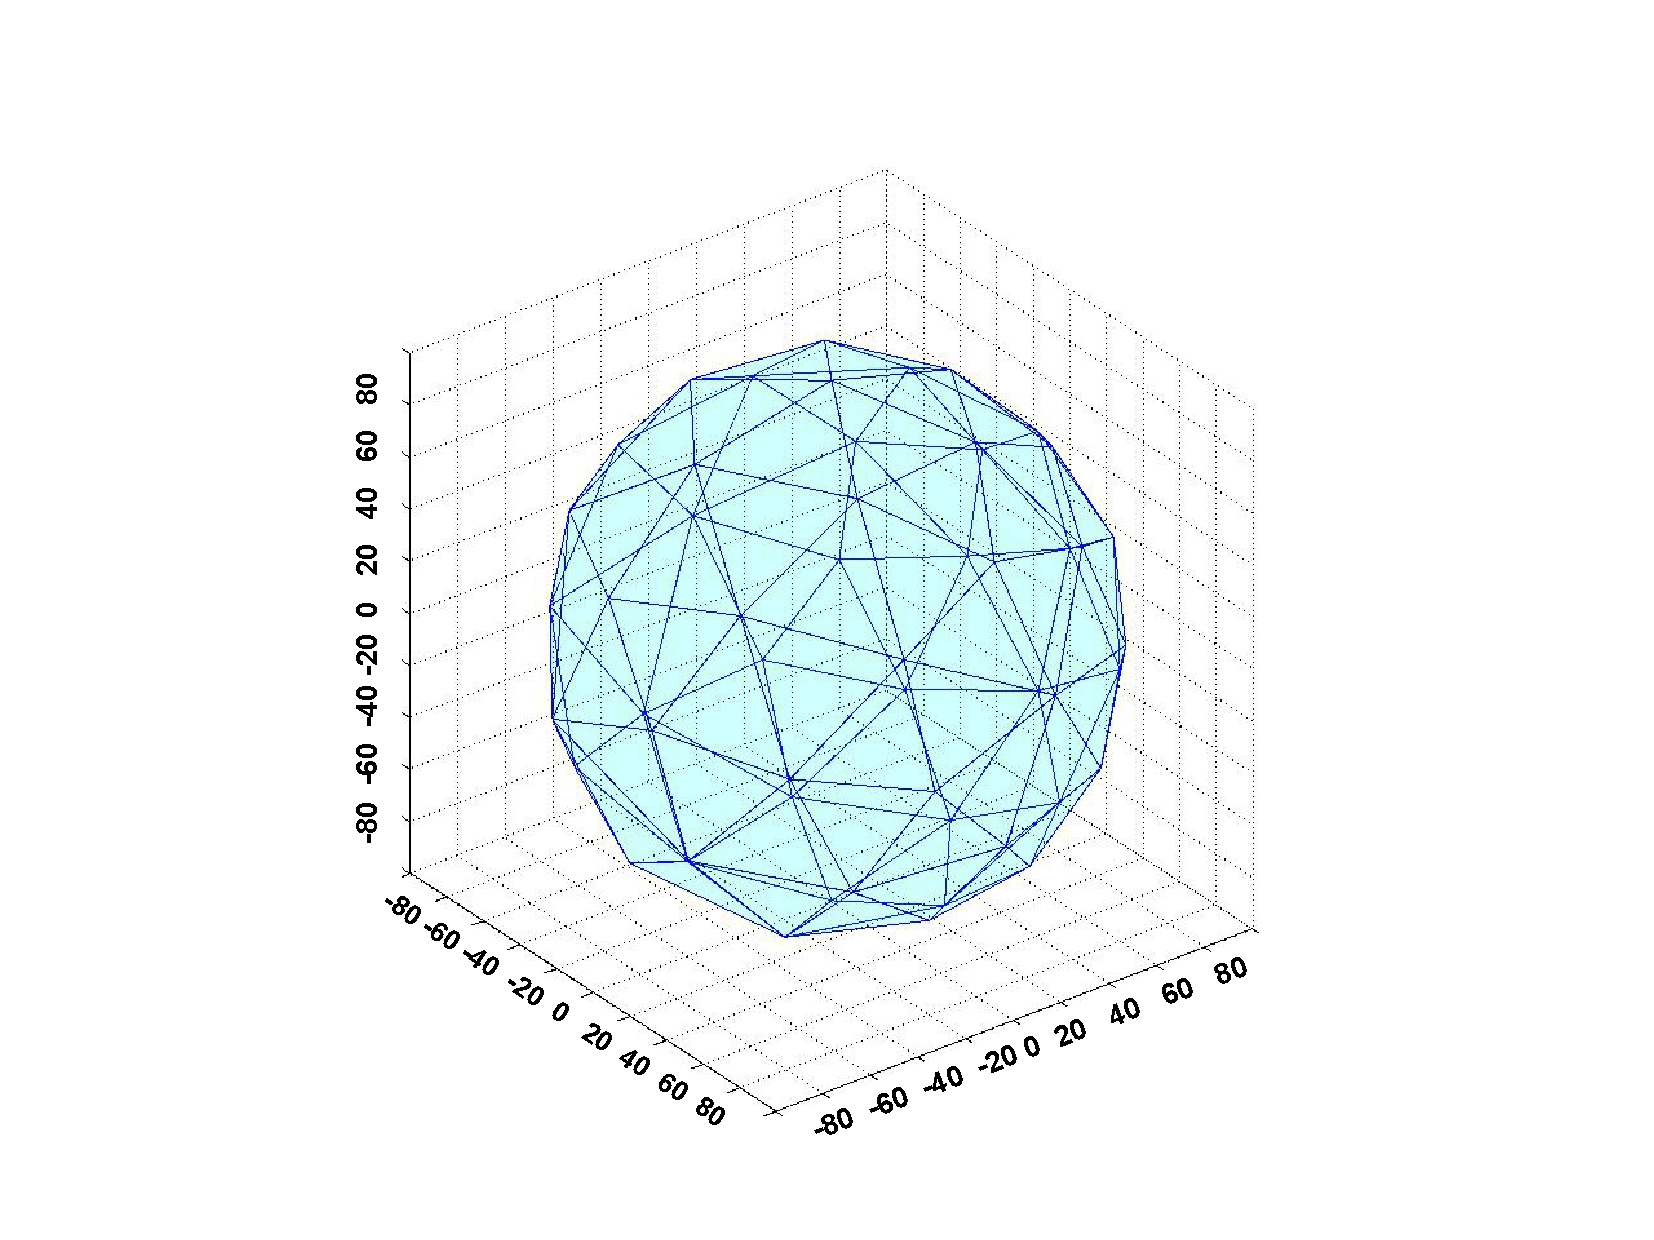
\includegraphics[height=2.5in,width=3.4in]{figures/NewSphere.pdf}
\centering 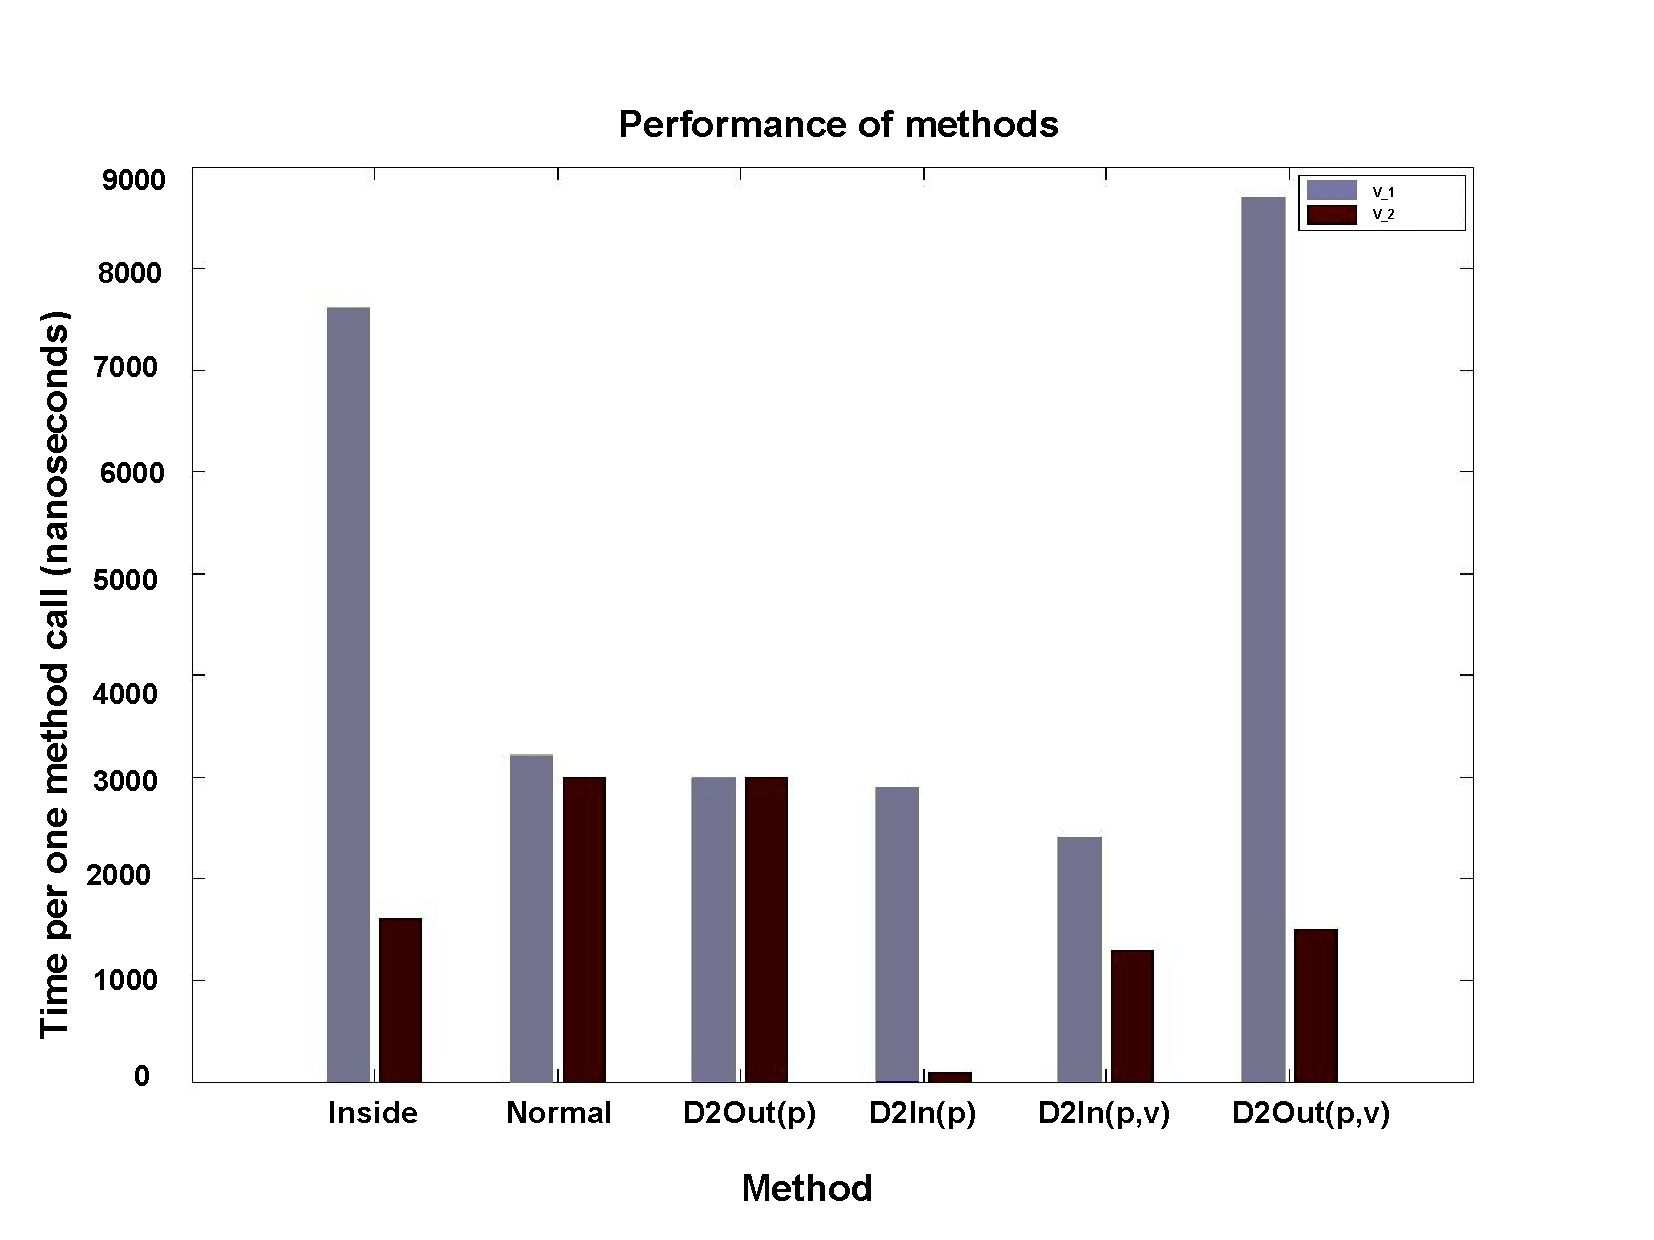
\includegraphics[height=3.4in,width=3.4in]{figures/tessellated_cpu.pdf}
\caption{Relative performance for the tessellated sphere (top), illustrated for
         each individual method.  Method name abbreviations are 
         D2In(p) : DistanceToIn(p), D2In(p,v) : DistanceToIn(p,v),
         D2Out(p) : DistanceToOut(p),  D2Out(p,v) : DistanceToOut(p,v).
         Light colored bars correspond to \Gfour{} 9.5.p02 and dark colored bars 
         correspond to \Gfour{} 9.6.p02.  Already for solids composed of a 
         relatively small number of facets (100 as in the case for the sphere), a 
         clear improvement is measured, especially for key methods.}
\label{tessellated_cpu}
\end{figure}
Since release 8.2 the geometry modeler has provided a tool to precisely identify
and flag defects in the geometry setup due to overlapping surfaces of physical 
volumes.  The technique makes use of the ability of each geometrical primitive
to randomly generate points lying on its surface and verifying that none of
these points is contained in other volumes of the same setup at the same level
in the geometry tree.  With the release 10 series, this technique is also used 
when ovelap checks are issued as UI commands, replacing the old method based on 
sampling over an overlapping grid of lines or cylinders.  These UI commands are 
listed and explained in section 4.1.11 (Detecting Overlapping Volumes) of the 
Application Developer Guide \cite{bib:AppDevGuide}.
% \begin{verbatim}
% /geometry/test/tolerance [double] [unit]
%   -- to define tolerance by which overlaps
%      should not be reported. Default is '0'.
% /geometry/test/verbosity [bool]
%   -- to set verbosity mode. Default is 'true'.
% /geometry/test/resolution [int]
%   -- to establish the number of points on
%      surface to be generated and checked for
%      each volume. Default is '10000'.
% /geometry/test/recursion_start [int]
%   -- to set the starting depth level in the
%      volumes tree from where checking 
%      overlaps. Default is level '0'.
% /geometry/test/recursion_depth [int]
%   -- to set the total depth in the volume 
%      tree for checking overlaps. Default
%      is '-1', which means checking the whole
%      tree.
% /geometry/test/maximum_errors [int]
%   -- to fix the threshold for maximum number
%      of errors to report for overlaps from a
%      volume. By default, for each volume,
%      reports stop after the first error
%      reported.
% /geometry/test/run
%   -- to start the overlaps checking
%      recursively through the volumes tree.
% \end{verbatim}

\subsubsection{Extensions to propagation in a field}
A gravitational field and the ability to create a force for it have been 
available in the toolkit since release 9.5.  Also, the force exerted on the 
magnetic moment in a gradient B-field is now taken into account for any 
particle, including neutrals.  An equation of motion was added that accounts for
the total combined force from magnetic, electric, gravitational and gradient 
B-fields as well as spin tracking.  With this it is possible to simulate the 
trajectory and spin of ultra-cold neutrons (UCN) and the trapping of neutral 
hydrogen atoms in a magnetic bottle.

A field can now be registered to a geometrical region, in addition to the global
reference frame or to a logical volume, as before.  

The mechanism to refine an intersection between a curved trajectory and volume 
boundaries was revised, making it possible to choose one of three methods or 
define a user-created method to do this.  A new multi-scale ``locator'' method 
(the new default), and a locator similar to Brent's method \cite{detmodeling:Brent} 
for root-finding, were added as alternatives to the original linear locator.
These allow the propagation in fields to cope with difficult trajectories which 
remain near to but just outside a curved surface.  This occurs in typical high 
energy physics applications which have nearly constant fields along the axis of
a tube.  The new methods also provide better overall CPU performance than the
old default, at the cost of more complex code.   

\subsubsection{Geometry persistency}
Detector geometrical descriptions can be imported and exported from text files
according to two different formats: the Geometry Description Markup Language 
(GDML)~\cite{MT:GDML} based on XML, or in plain ASCII text.  \Gfour{} provides
internal modules which allow the interpretation and conversion of the above 
formats to and from the internal geometry representation, without the need for 
C++ programming for the implementation of the various detector description 
setups.

\subsubsection*{GDML geometry}

In version 3 of GDML, the part of GDML I/O which provides the ability to
export and import detector geometry descriptions to and from GDML files, was
integrated into \Gfour{} by means of the GDML module making use of the DOM
XML parser provided with the Xerces-C++~\cite{detmodeling:XercesC} software
package.

The \Gfour{} binding for GDML implements all features supported by the \Gfour{}
geometry modeler and most of the geometrical entities defined as part of the
latest version of the GDML schema. These include all shapes, either CSG or 
specific solids, and their boolean combinations.  Also included are any 
combinations of materials, from isotopes to mixtures, and the ability to import
definitions compliant with the \Gfour{} NIST database.

All types of physical volumes are supported, from placed volumes to replicas and
parameterized volumes, including assemblies, divisions and reflections.

GDML supports the modularization of geometry descriptions to multiple GDML
files, allowing for rational organization of the modules for complex setups.
Verification of the GDML file against the latest version of the schema comes
for free thanks to Xerces-C++, with the possibility to turn it on or off in
the \Gfour{} GDML parser.

Recent additions to the GDML parser enable efficient import/export of 
tessellated solids, and the treatment of parameterizations for polycones, 
polyhedra and ellipsoids.  Release 10.1 of \Gfour{} provides support for the
definition, import and export of multi-union structures when making use of the
Unified Solids library.

Several examples are provided to illustrate most of the features of the 
\Gfour{} GDML parser:
\begin{verbatim}
examples/extended/persistency/gdml/G01
examples/extended/persistency/gdml/G02
examples/extended/persistency/gdml/G03
examples/extended/persistency/gdml/G04  .
\end{verbatim}
Example G01 shows how to write a simple application for importing and exporting
GDML files, providing a variety of samples for different kinds of solids, 
volumes, material descriptions, integration of optical surface parameters, and
so on.  Example G02 demonstrates how to import/export different geometry setups,
including STEP Tools \cite{detmodeling:STEPTools} files and structures, 
integrating them into a real simulation application.  In example G03 it is shown
how to define and import extensions to the GDML schema for attributes associated 
with a logical volume.  G04 is a simple example showing how to associate 
detector sensitivity with a logical volume, making use of the GDML feature for 
defining auxiliary information.

\subsubsection*{ASCII geometry}

The format of the ASCII text file is based on the use of tags: special words at
the beginning of each line setting what the line is describing. 

With this format the user may describe any of the geometrical objects of \Gfour{}.
It is possible to create materials combining elements, materials and detailed
isotopic composition.  Mixtures of materials can be built by providing the 
percentage of each material by weight, by volume or by giving the number of 
atoms.  The user may change the default pressure, temperature and state, or set
the minimum ionizing energy instead of letting \Gfour{} calculate it 
automatically.  Instead of explicitly building each material, predefined 
elements or materials from the \Gfour{} NIST database may be specified.
% which includes all elements from Z=1 to Z=107,
% all single-element materials from Z=1 to Z=98 and more than 200 other material
% compositions.

% \begin{figure}
%  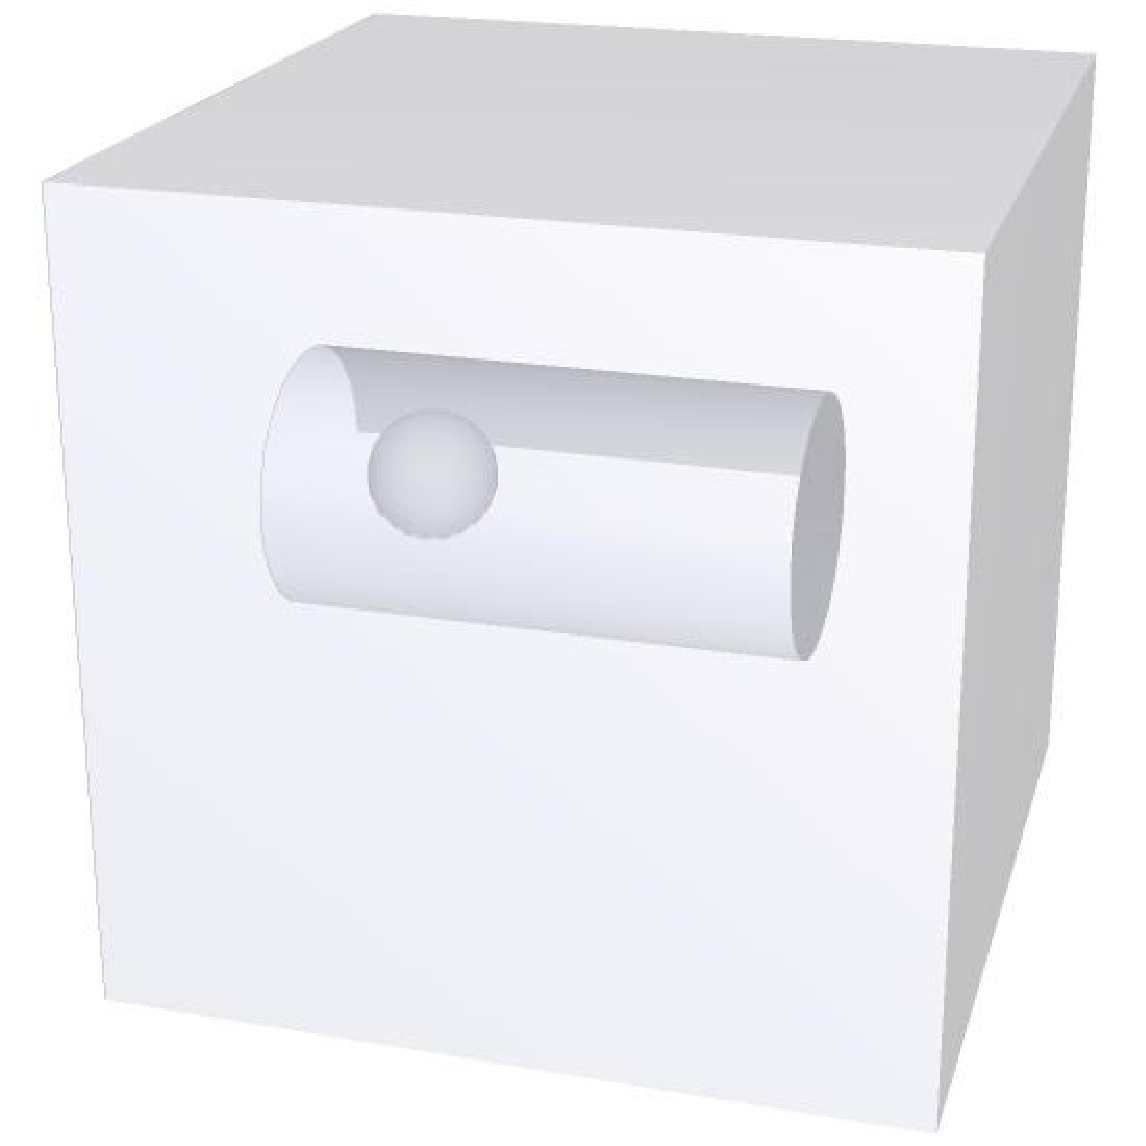
\includegraphics[width=0.45\textwidth]{figures/ascii_example.pdf}
% \caption{Geometry setup corresponding to the ASCII specification given in the text.}
% \label{ascii_example}
% \end{figure}

Most types of \Gfour{} solids can be described, whether CSG or specific, by
including a combination of solids through boolean operations.  Logical volumes
can be defined by attaching solids to materials, and color and visualization 
attributes can be assigned to each one.  After building the logical volumes, 
they can be placed individually or by using replicas, divisions, assemblies or
parameterizations.  As it is almost impossible with a scripting language to 
cover all the possible parameterizations a user may need, only the most common
ones are available: linear, circular, square or cubic.  If others are needed,
it is possible to define them through C++ code and mix them with the rest of
the geometry in ASCII format.  To place the volumes, rotation matrices can be
defined with three different formats providing: values of the three rotation 
angles about the three axis, the theta and phi angles that define the 
orientation of the three axes, or the elements of the 3$\times$3 rotation
matrix. 

\begin{figure}
    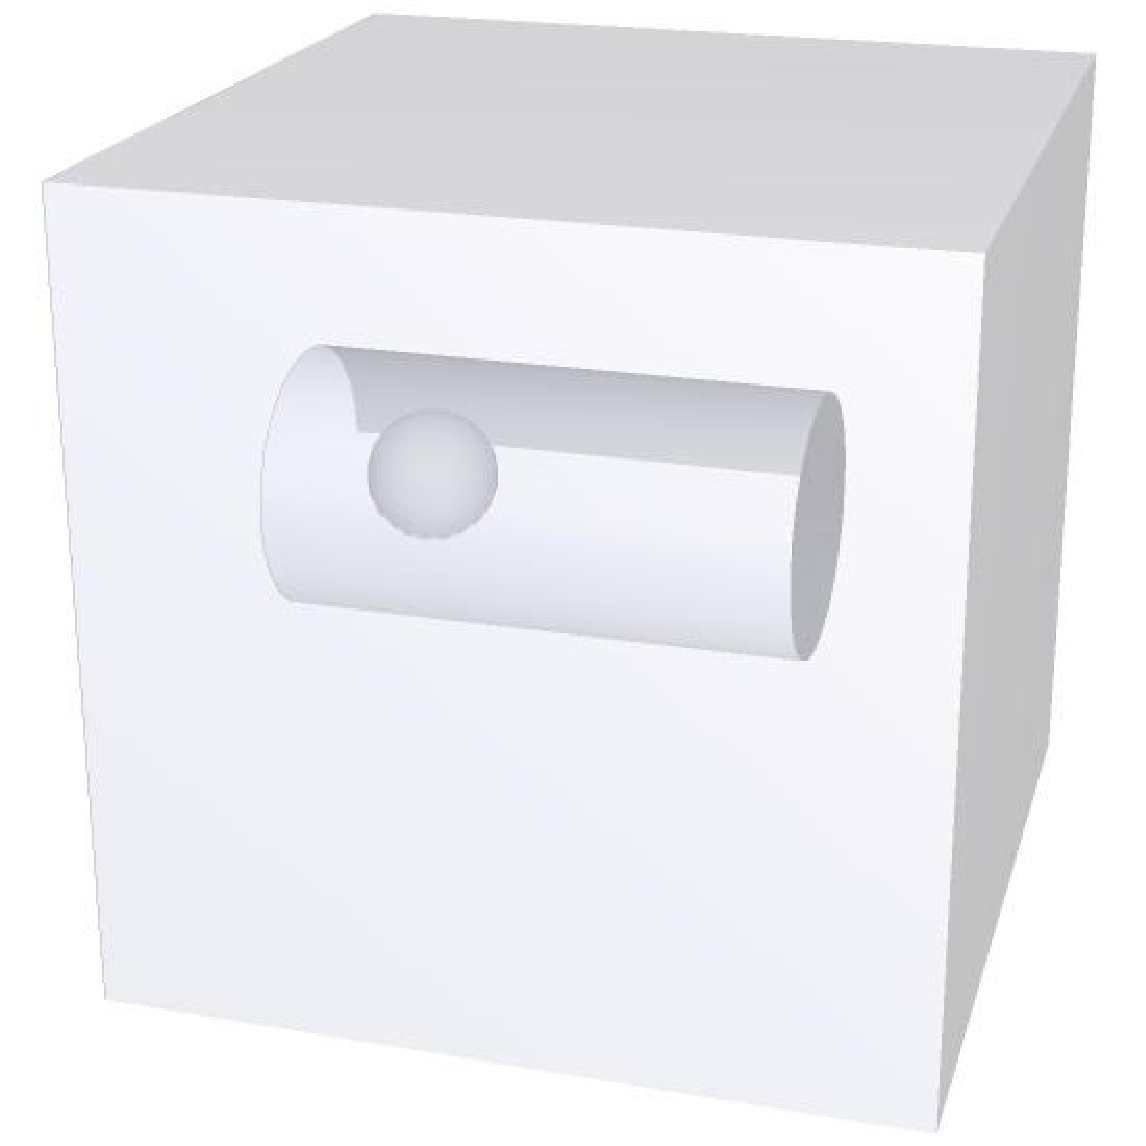
\includegraphics[width=0.45\textwidth]{figures/ascii_example.pdf}
\caption{Geometry setup corresponding to the ASCII specification given in the text.}
\label{ascii_example}
\end{figure}

To facilitate the definition of a complex geometry, it is possible to use
parameters: values that can be assigned to keywords, so that they can be reused
later in any part of the geometry.  It is also possible to define numerical 
values through arithmetic expressions.
%, like
% \begin{verbatim} 
% (cos(3.)*3./sqrt(5.)) .
% \end{verbatim}
The code automatically assigns a default unit depending on the dimension: mm,
degrees, MeV, nanoseconds, $g/cm^3$, but the user may change it at any place.
Comments may be used at any point in the file, using the C++ style of placing
two forward slashes before the comment.

If the geometry description is long, it may be split into several files, which
may be combined by setting a
% \verb{#include} tag. It is also possible to
\begin{verbatim}
#include
\end{verbatim}
tag.  It is also possible to combine part of the geometry with C++ code and
another part with ASCII format.  If the user has a geometry already defined in
C++, it may be transformed into ASCII format by adding a user action in the
code.

The text format is thoroughly checked and clear error messages are provided 
when necessary.  Arithmetic expressions are checked for correctness and the 
parameters in each tag are compared against expected number and type.  An error 
message results if a line refers to a non-existent element.

An example of the geometry ASCII text format is given here and the resulting
picture is shown in Figure \ref{ascii_example}:

\begin{verbatim}
// Define a parameter for later use
:P DIMZ 5.

// Define materials
:ELEM Hydrogen H 1. 1.
:ELEM Oxygen O 8 16.
:ELEM Nitrogen N 7 14.
:MIXT Air 1.214E-03 2
      Nitrogen   0.75
      Oxygen     0.25

// Define rotation matrix
:ROTM R00  0. 0. 0.  // unit matrix

// Define volumes and place them
:VOLU world BOX 30. 30. 30. Air

:VOLU "my tube" TUBE 0. 10. $DIMZ*4 G4_WATER
:PLACE "my tube" 1 world R00 0. 0. $DIMZ

:VOLU sphere ORB 5.  G4_AIR
:PLACE sphere 1 "my tube" R00 0. 1. 10.
\end{verbatim}

% \begin{figure}
%     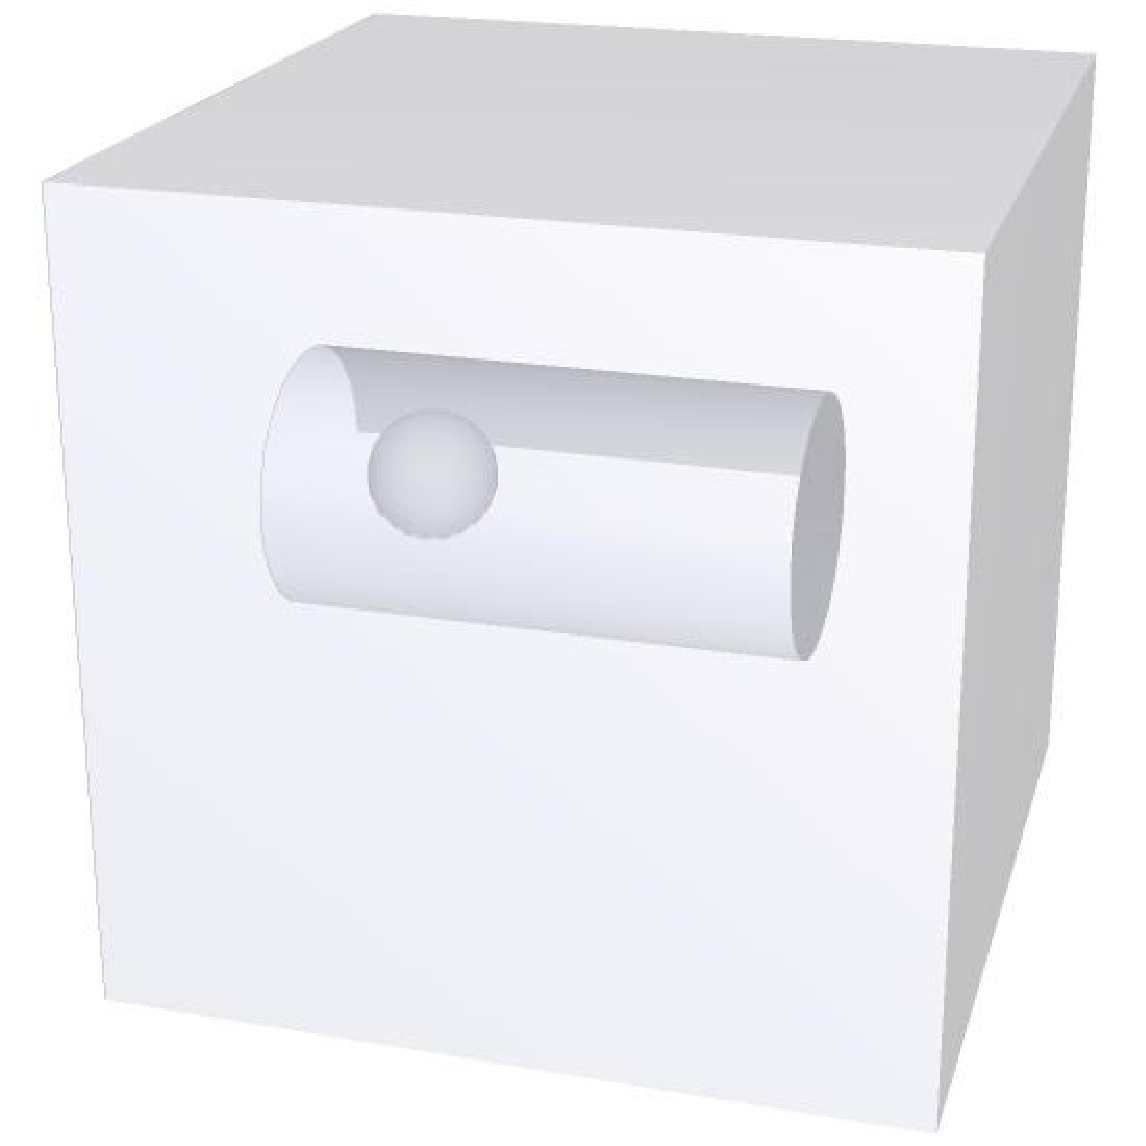
\includegraphics[width=0.45\textwidth]{figures/ascii_example.pdf}
% % \centering 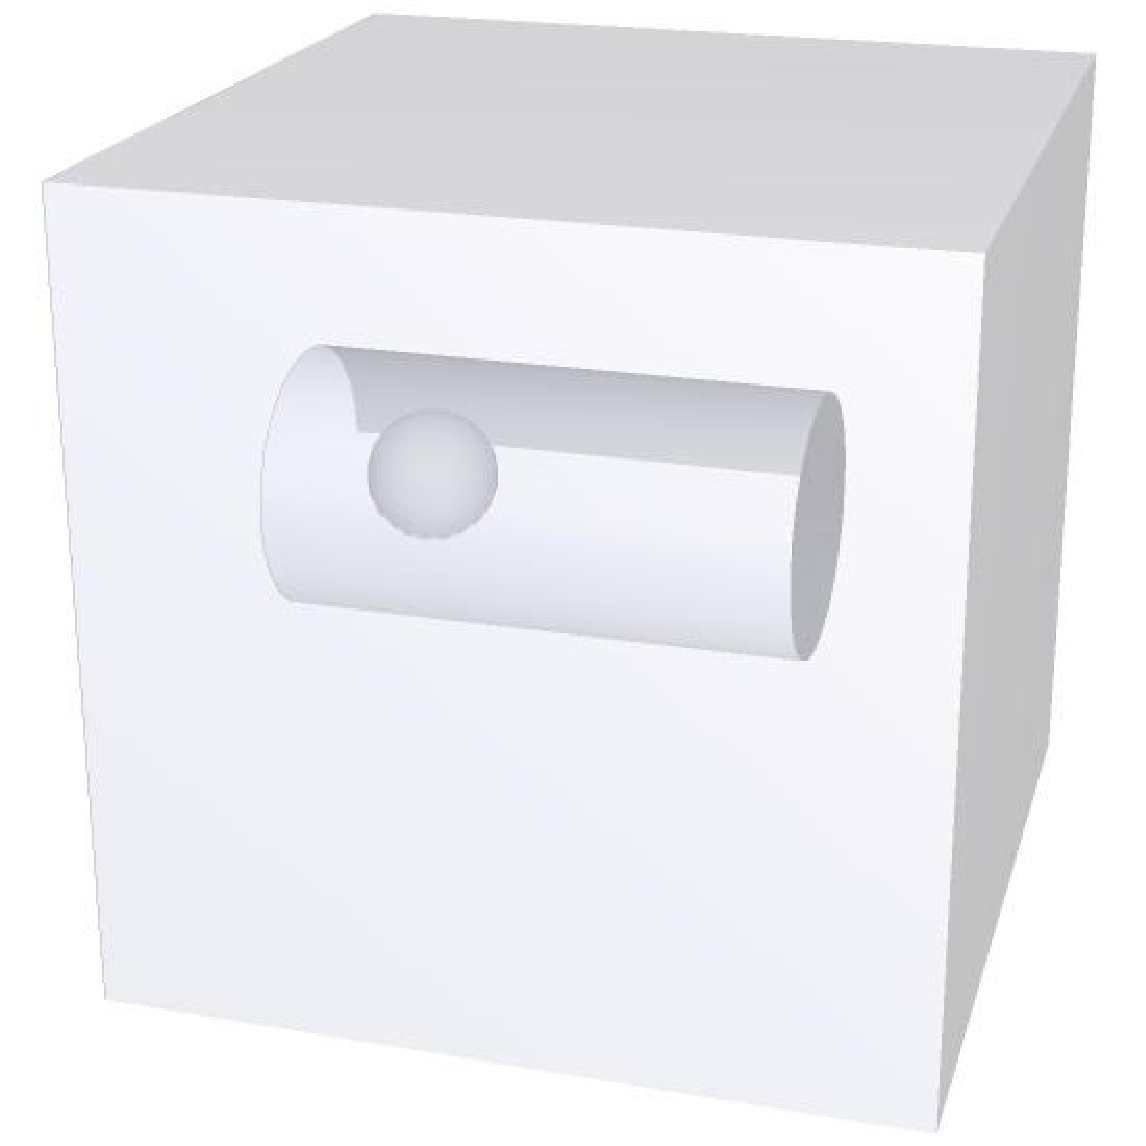
\includegraphics[height=2.8in,width=3.0in]{figures/ascii_example.pdf}
% \caption{Geometry corresponding to the ASCII text file above.}
% \label{ascii_example}
% \end{figure}

An example, \verb"examples/extended/persistency/P03", is included with the 
\Gfour{} distribution to illustrate the use of the ASCII text geometry.  Several
text geometry files are provided to illustrate the many different geometry
construction options.
% possibilities:
% \begin{itemize}
% \item simple construction of materials and single placements, 
% \item isotopes, elements and materials,
% \item boolean solids,
% \item reflections,
% \item replicas,
% \item divisions,
% \item linear parameterizations,
% \item square parameterizations and
% \item assembly placements.
% \end{itemize}   	
This example also shows how to define a sensitive detector, mix C++ code with
ASCII files, extend the format to create a new tag and dump the in-memory 
geometry to an ASCII file.

% \subsubsection{Multithreading implications}
% Geometry objects are shared.
% [John, Makoto]
% Implications for user code and how to organize detector construction.
% [John, Makoto, Andrea]
